% 2021 全国甲卷文科 23：供考生作图用的空白方格坐标系
% 绘制依据：源 PDF 第 2 页原图。整幅为方格网，坐标轴过原点，
% 原点偏右下（左侧格数多于右侧，上方格数少于下方），仅标注 O 与两轴上的 1。
% 本图无曲线内容——它是题目要求「画出 y=f(x) 和 y=g(x) 的图象」的作图区。
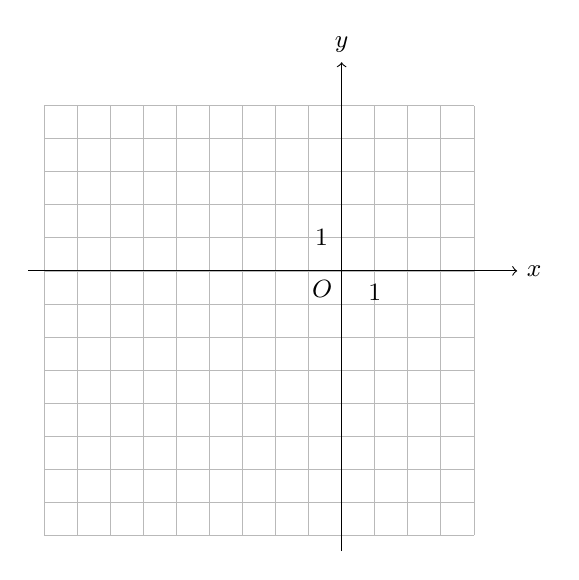
\begin{tikzpicture}[font=\small, line width=0.4pt]
  \def\u{0.42}% 单位格边长
  \pgfmathsetmacro{\xa}{-9}\pgfmathsetmacro{\xb}{4}
  \pgfmathsetmacro{\ya}{-8}\pgfmathsetmacro{\yb}{5}
  % 方格网
  \draw[gray!55, line width=0.25pt] ({\xa*\u},{\ya*\u}) grid[step=\u] ({\xb*\u},{\yb*\u});
  % 坐标轴
  \draw[->] ({\xa*\u-0.20},0) -- ({\xb*\u+0.55},0) node[anchor=west] {$x$};
  \draw[->] (0,{\ya*\u-0.20}) -- (0,{\yb*\u+0.55}) node[anchor=south] {$y$};
  % 标注
  \node[anchor=north east, inner sep=2pt] at (-0.04,-0.04) {$O$};
  \node[anchor=north,      inner sep=3pt] at ({1*\u},-0.06) {$1$};
  \node[anchor=east,       inner sep=3pt] at (-0.06,{1*\u}) {$1$};
\end{tikzpicture}
